\chapter{Introduction}
\label{chap:intro}

\section{Background}

Computer networks contain two types of nodes: the {\em end hosts} that generate
packets and the {\em routers}\footnote{We use the term router to refer to both
switches and routers in this dissertation.} that forward these packets between
the end hosts. Historically, the Internet was architected so that most of the
complexity resided in the end hosts, while the routers themselves were simple.
According to Clark~\cite{design_philosophy}, this architecture was a result of
the primary design goal of the Internet: the ability to easily interconnect a
diverse set of existing networks (\eg long-haul networks, local-area networks,
satellite networks, and radio networks). Quoting Clark, "The Internet
architecture achieves this flexibility by making a minimum set of assumptions
about the function which the net will provide."

The minimum functionality assumed of and provided by the network was
best-effort and unreliable packet forwarding. Notably absent from a router's
feature set were reliable packet delivery, packet prioritization, monitoring
features to attribute a router's resource usage to specific end hosts, and
security features to detect network breaches. As a result, the early routers
were singularly dedicated to packet forwarding. A minimal router feature set
made it simpler to design high-speed routers and helped broaden the Internet's
reach by interconnecting existing networks with minimum friction. But, it
sidelined other goals~\cite{design_philosophy} such as improving network
performance, security, and monitoring.
 
Today, four decades after ideas underlying the Internet were first
published~\cite{cerf74}, it is clear that routers need to do much more than
forward packets for at least two reasons. First, once the basic goal of
interconnecting different networks is achieved, other goals like performance,
security, and monitoring rise in prominence.  Second, many large-scale private
networks (\eg datacenters, private wide-area networks, enterprise networks) do
not need to concern themselves with interconnecting diverse networks as the
Internet had to---and hence can expect more from their network. As a result, a
typical router today implements many features beyond packet forwarding,
pertaining to security (\eg access control), monitoring (\eg counting the
number of packets belonging to each flow), and performance (\eg priority
queues).

While a router's functionality has steadily increased with time, there's little
consensus between network operators and router vendors on a router's feature
set. Inevitably, there are network operators whose needs fall outside their
router's feature set. But because today's fastest routers are built out of
specialized forwarding hardware, they are largely {\em
fixed-function}\footnote{The term fixed-function was first used to describe
graphics processing units (GPUs) with limited or no
programmability~\cite{gpu_fixed}. We use it in an analogous sense here.} in the
sense that their functionality cannot be changed once the router has been
built. In such cases, the operator has no alternative but to wait two--three
years for the next generation of the router hardware. This is best illustrated
by the lag time between the standardization and availability of new overlay
protocols~\cite{nvgre}.

As a result, the rate of innovation in new router algorithms is outstripping
our ability to get these algorithms into production routers, \ie routers that
are seen in the wild today and have aggregate speeds in the several hundred
Gbit/s to Tbit/s range.  Figure~\ref{fig:router_algos} shows a timeline of
prominent router algorithms that have been developed since the 1980s. Of these,
only a handful are available in production routers because there is no way to
program a new router algorithm on these routers.
%TODO: Maybe give examples of production routers. 

\begin{figure}
\centering
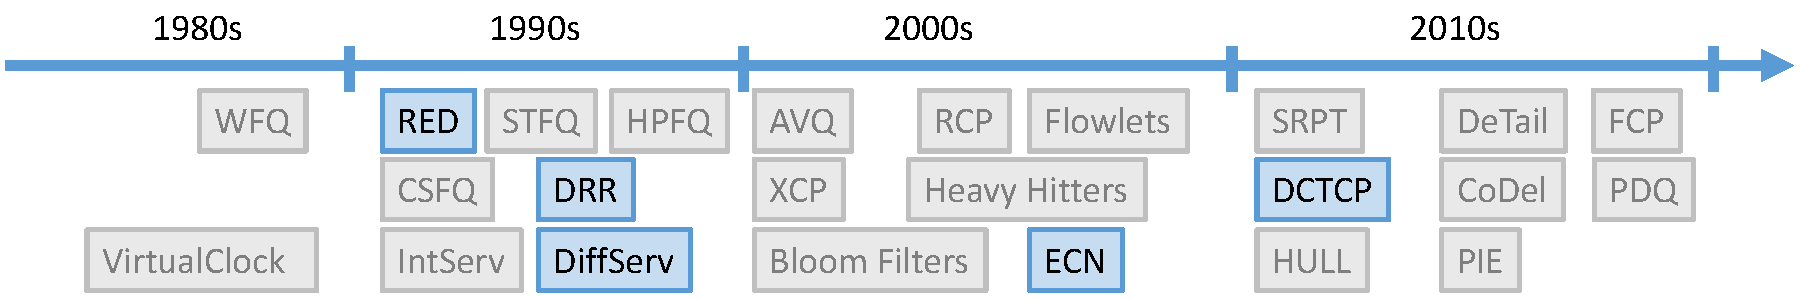
\includegraphics[width=\columnwidth]{router_alg_timeline.pdf}
\caption{Timeline of prominent router algorithms since the 1980s. Only the ones
shaded in blue are available on production routers today.}
\label{fig:router_algos}
\end{figure}

For an operator wanting to introduce new functionality in their network, what
are the operator's choices? One is to give up on changing routers altogether
and make all the required changes at the end hosts.  Relying solely on the end
hosts, however, results in cumbersome or suboptimal solutions. As a first
example, imagine measuring the queuing latency at a particular hop in the
network. One could do this by collecting end-to-end ping measurements between a
variety of vantage points and then fusing these measurements together to
estimate per-hop queueing latency. Not only is this indirect, it is also
inaccurate relatively to directly instrumenting the router at that hop to
measure its own queueing latency. As a second example, consider the problem of
congestion control, which divides up a network's capacity fairly among
competing users. There are many in-network solutions to congestion
control~\cite{xcp, rcp}, which outperform the end-host-only approaches to
congestion control used today~\cite{cubic, compound}. But, there is no way to
deploy them.

Another alternative is to use a \textit{software router}: a catch-all term for
a router built on top of some programmable substrate, such as a general-purpose
CPU~\cite{click, routebricks}, a network processor\footnote{A CPU with an
instruction set tailored to packet processing~\cite{ixp4xx, ixp2800}.}, a
graphics processing unit (GPU)~\cite{packetshader}, or a field-programmable
gate array (FPGA)~\cite{netfpga}.  Figure~\ref{fig:router_evolution} tracks the
evolution of aggregate capacity of software routers and compares them to the
fastest routers known at any point in time. The figure shows two trends.
First, until the mid 90s, software routers were in fact the fastest routers;
the early routers~\cite{imp} were minicomputers loaded with forwarding
software. Second, since the mid 90s, growing demands for higher link speeds,
fueled by the Internet's growth, have meant that the fastest routers are now
built out of dedicated hardware, specialized for packet forwarding.
%TODO: More examples of early routers ...

Hardware specialization gives these routers a 10--100 $\times$ performance
improvement relative to software routers.  This performance improvement is the
result of fully exploiting the abundant parallelism available in packet
processing. First, data parallelism, the ability to simultaneously process
either different parts of the same packet or packets belonging to different
ports. Second, pipeline parallelism, the ability to simultaneously perform
different operations on different packets. But, hardware specialization carries
a cost: because routers are built out of specialized hardware, they are
fixed-function devices that can not be reconfigured in the field.

Recent work in software-defined networking~\cite{openflow} (SDN) and
programmable switching chips~\cite{rmt, xpliant, flexpipe} has endowed fast
routers with limited flexibility. SDN allows operators to program the network
control plane, which is the part of the network that computes a network's
routing tables, by moving route computations out of the routers and on to a
programmable server. Programmable switching chips allow operators to program
parts of the data plane, which is the part of the network that forwards packets
based on the routing tables, such as packet header manipulations that do not
modify router state.  However, these solutions are still not sufficient to
express the grayed-out algorithms shown in Figure~\ref{fig:router_algos}
because (1) these algorithms programmatically manipulate router state and (2)
they require flexibility in packet scheduling, which is untouched by both SDN
and programmable switching chips.

\begin{figure}
\centering
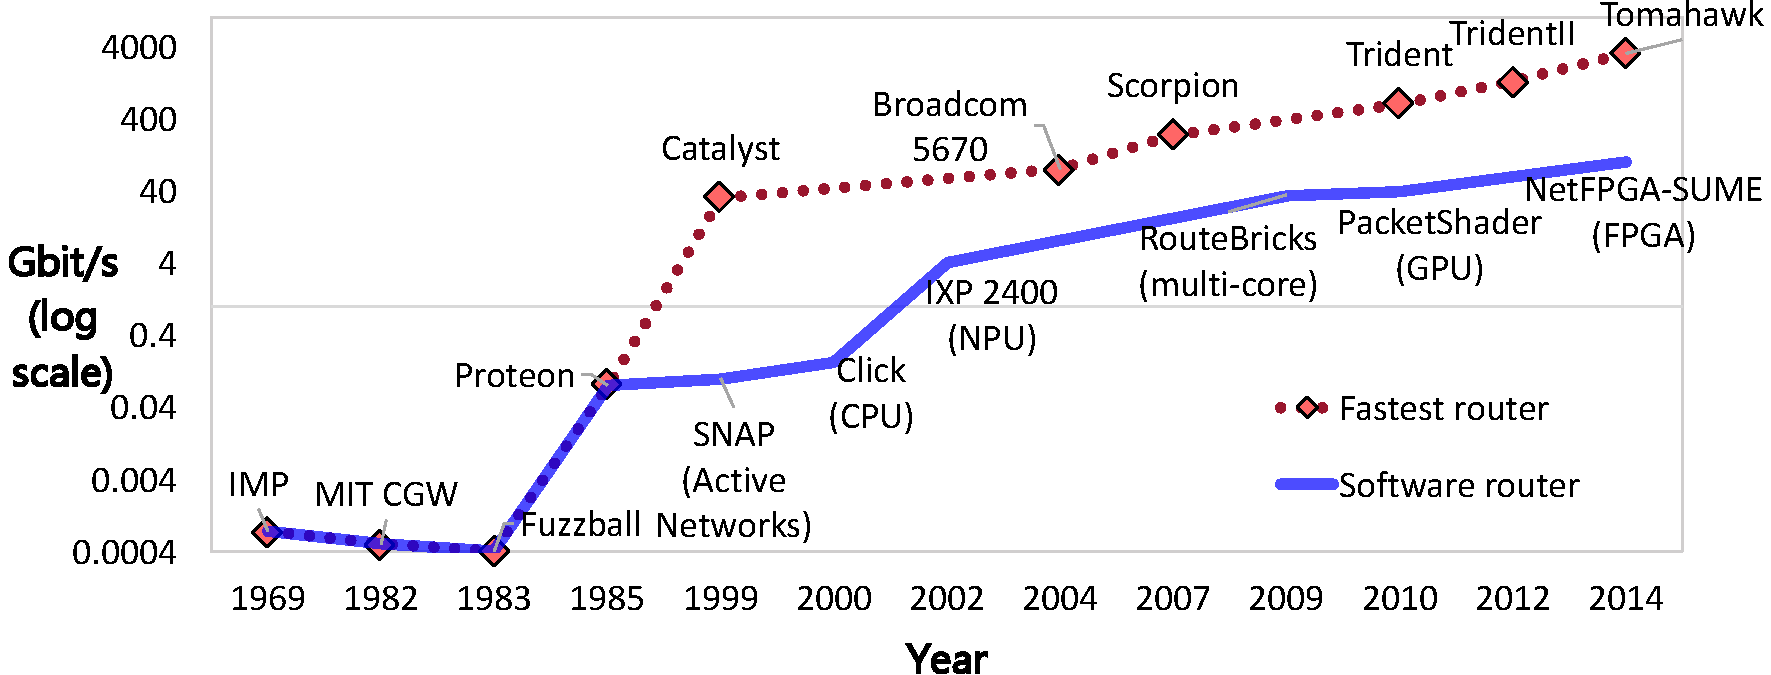
\includegraphics[width=\columnwidth]{router_evolution.pdf}
\caption{Aggregate capacity of routers since the first router on the ARPANET in
1969~\cite{imp}. Until the mid 90s, software routers were sufficient. Since
then, however, the fastest routers have been built out of dedicated hardware.}
\label{fig:router_evolution}
\end{figure}

\section{Primary contributions}
\begin{table}
\textbf{Stateful data-plane algorithms (Chapter~\ref{chap:domino})}
\\[-7pt]\rule{\textwidth}{1pt}\\[-7pt]\rule{\textwidth}{1pt} \\
\textbf{Examples:} In-network congestion control (\eg XCP~\cite{xcp} and
RCP~\cite{rcp}), active queue management (\eg RED~\cite{red}, BLUE~\cite{blue},
and CoDel~\cite{codel}) \\
\textbf{Technical challenge:} How do we allow programmable router state
modification at the router's line rate, when a new packet can be received as
often as every nanosecond? \\
\textbf{Programming model:} Packet transactions (\S\ref{s:transactions})\\
\textbf{Hardware primitive:} Atoms (\S\ref{s:absmachine}) \\
\textbf{Key finding:} A small set of atoms (Table~\ref{tab:templates}) is
simultaneously (1) expressive enough to serve as the instruction set for many
stateful algorithms (Table~\ref{tab:algo_atoms}) and (2) feasible
in high-speed hardware (\S\ref{s:eval}). Further, we find that these atoms
can support several new use cases that were unanticipated at the time the atoms
were designed (Table~\ref{tab:atoms_generalize}).\\ \\

\textbf{Scheduling algorithms (Chapter~\ref{chap:pifo})}
\\[-7pt]\rule{\textwidth}{1pt}\\[-7pt]\rule{\textwidth}{1pt} \\
\textbf{Examples:} Weighted Fair Queueing~\cite{wfq} and priority scheduling~\cite{srpt} \\
\textbf{Technical challenge:} Can we find an abstraction that unifies many disparate
scheduling algorithms? \\
\textbf{Programming model:} Scheduling trees (\S\ref{s:pifo}) \\
\textbf{Hardware primitive:} A priority queue data structure called a Push In First Out
Queue (PIFO) (\S\ref{s:design}) \\
\textbf{Key finding:} A priority queue of packets with a program to set each
packet's priority can express many scheduling algorithms
(\S\ref{s:expressive}) and is feasible in high-speed hardware
(\S\ref{s:hardware}). \\\\

\textbf{Scalable per-flow statistics (Chapter~\ref{chap:perf_query})}
\\[-7pt]\rule{\textwidth}{1pt}\\[-7pt]\rule{\textwidth}{1pt} \\
\textbf{Examples:} Per-flow measurements of moving averages, counters, and loss rates \\
\textbf{Technical challenge:} Can we allow programmers to flexibly define the
per-flow statistics they want to measure and also scale these measurements to a large number of
flows?\\
\textbf{Programming model:} Performance queries (\S\ref{sec:language}) \\
\textbf{Hardware primitive:} Programmable hardware key-value store. Keys correspond to
flows and values to statistics. (\S\ref{sec:aggregation}) \\
\textbf{Key finding:} A class of statistics measurements, which we call the
linear-in-state class (\S\ref{sec:linear-in-state-description}), can be scaled
to a large number of flows without losing accuracy. This class covers many
practically useful statistics such as counters, moving average filters, and
conditional counters (\S\ref{sec:eval}). \\
\caption{Contributions of this dissertation}
\label{tab:contributions}
\end{table}


This dissertation considers the problem of building routers that approach the
speeds of today's fastest fixed-function routers, while also being
programmable. My thesis is that {\em it is possible to design router hardware
that is both fast and programmable, if we restrict ourselves to programming
specific classes of router functionality}. It is this specificity that allows
us to resolve the programmability-performance tension; indeed, our designs
provide a much more restricted form of programmability than a Turing-complete
processor.  The challenge here is to pick classes of router functionality that
are simultaneously (1) practically useful to network operators, (2) broad
enough to cover a range of current and future use cases within that class, and
yet (3) narrow enough to permit a high-speed hardware implementation. We will
describe high-speed programmable hardware primitives and their corresponding
programming models in software for three classes of router functionality:
stateful data-plane algorithms, packet scheduling, and scalable network
measurement.  Table~\ref{tab:contributions} summarizes our contributions.

\subsection{Stateful data-plane algorithms}
In Chapter~\ref{chap:domino}), we consider the problem of programming {\em
stateful data-plane algorithms} at high packet processing rates. These are
algorithms that operate on a sequeunce of packets in a streaming manner, doing
a bounded amount of work per packet and manipulating a bounded amount of router
state in the process.  They include algorithms for managing the router's buffer
(\eg RED~\cite{red}, BLUE~\cite{blue}), load balancing (\eg CONGA~\cite{conga},
flowlet switching~\cite{flowlets}), and in-network congestion control (\eg XCP~\cite{xcp},
RCP~\cite{rcp}).

High-speed data-plane programming poses two challenges: (1) what hardware
instructions are required to support programmable state modification at the
router's line rate and (2) what is the right programming model? To address
these challenges, we develop a system for data-plane programming, Domino, which
contains three main components: an instruction set (atoms), a programming model
(packet transactions), and a compiler.

\Para{Atoms.} \textit{Atoms} capture a router's instruction set. They specify
atomic units of packet processing provided by the router hardware, \eg an
atomic counter or an atomic test-and-set. Figure~\ref{fig:simple_atom} shows an
example atom. Atoms are atomic in the sense that if some state is updated by an
atom as part of processing a packet, the next packet arriving at that atom will
see the updated value of that state. The processing within atoms is constrained
to meet the atomicity requirement by ensuring that the input-to-output latency
of the atom's digital circuit is under a clock cycle, so that the output is
updated to the correct value in time for the next packet arriving at the atom a
clock cycle later.

\Para{Packet Transactions.} \textit{Packet transactions} provide a programming
model for data-plane algorithms. A packet transaction is an atomic and isolated
block of code capturing an algorithm's logic written in a domain-specific
language (DSL) called Domino. Figure~\ref{fig:simple_transaction} shows an
example packet transaction.  Packet transactions provide programmers with the
illusion that the transaction's body executes serially from start to finish on
each packet, with no overlap in packet processing across packets---akin to an
infinitely fast single-threaded processor carrying out packet processing on
each packet. Packet transactions are expressive and capture many important
data-plane algorithms.  Further, their serial semantics shield programmers from
the router's data and pipeline parallelism.
%%Packet transactions have been
%%adopted in P4~\cite{p4}, a packet-processing language that is emerging as an
%%industry standard for programming router chips.  P4 programmers can now use an
%%@atomic annotation around a block of statements to specify that the block must
%%execute atomically.

\Para{The compiler.} The Domino compiler compiles packet transactions written
in the Domino DSL to a pipeline of atoms provided by the router, and rejects
the code if the router's atoms cannot support the packet transaction.

The compiler has three phases (Figure~\ref{fig:compiler_passes_example}). First
(\S\ref{ss:preprocessing}), it preprocesses the code to make it easier to infer
dependencies between packet-processing operations. Second
(\S\ref{ss:pipelining}), the compiler then transforms the preprocessed, but
still serial, packet transaction into a parallel pipeline of {\em codelets}.
When pipelining, the compiler maintains the invariant that if each codelet
executes atomically and passes off its results to the next codelet, the
behavior will be indistinguishable from the packet transaction itself executing
atomically on each packet. Third (\S\ref{ss:code_gen}), the compiler maps each
codelet one-to-one to an atom provided by the underlying router, rejecting the
code if the codelet cannot be supported by the atom.

The compiler provides an {\em all-or-nothing} guarantee: if the compiler
compiles the packet transaction it will run at the line rate of the router; all
other programs that cannot run at line rate---because there isn't an atom to
carry out the program's operations at line rate---will be rejected. A
conventional compiler for a general-purpose CPU compiles all programs, but a
program's run-time performance depends on its complexity. In Domino, only
programs that are simple enough to run at the router's line rate will be
compiled, obviating the need for any performance profiling.

\Para{Evaluation.}
Developing atoms for a router is a chicken-and-egg problem. A router's atoms
determine what algorithms the router can support, while the algorithms
determine what atoms are required in the first place. Designing the right atoms
is especially important for a programmable line-rate router because---unlike a
general-purpose CPU---there is no way to ``emulate'' functionality in software
when hardware support is not available.

\begin{figure}[!t]
\begin{minipage}{0.48\textwidth}
\centering
\vspace{0.38in}
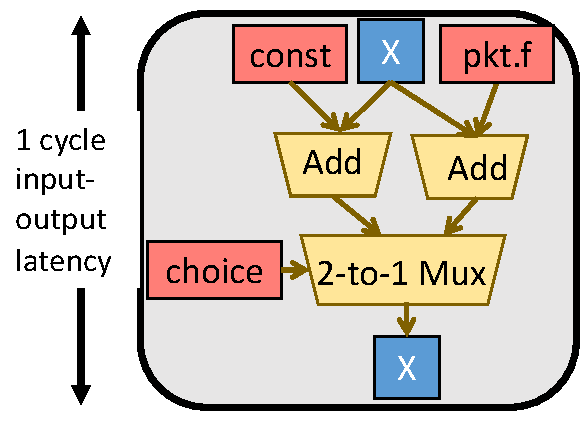
\includegraphics[width=0.85\textwidth]{atom.pdf}
\caption{An atom that either adds either a constant or a packet field to a
piece of state x and writes it back to x.}
\label{fig:simple_atom}
\end{minipage}
\hfill
\begin{minipage}{0.48\textwidth}
\centering
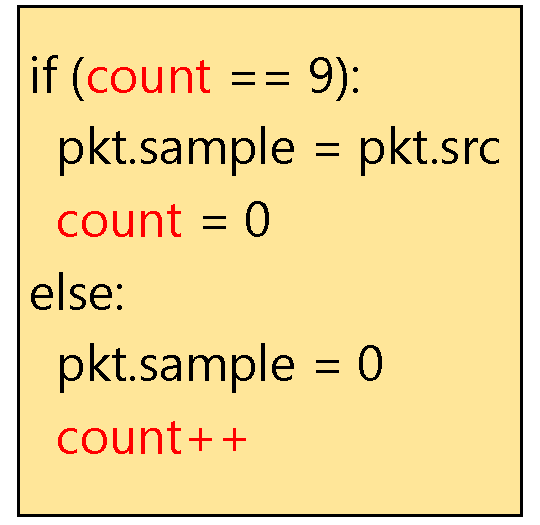
\includegraphics[width=0.75\textwidth]{packet_transaction.pdf}
\caption{A packet transaction that samples the src IP address of every 10th
packet. State variables (count) are in red.}
\label{fig:simple_transaction}
\end{minipage}
\end{figure}

\begin{figure}[!t]
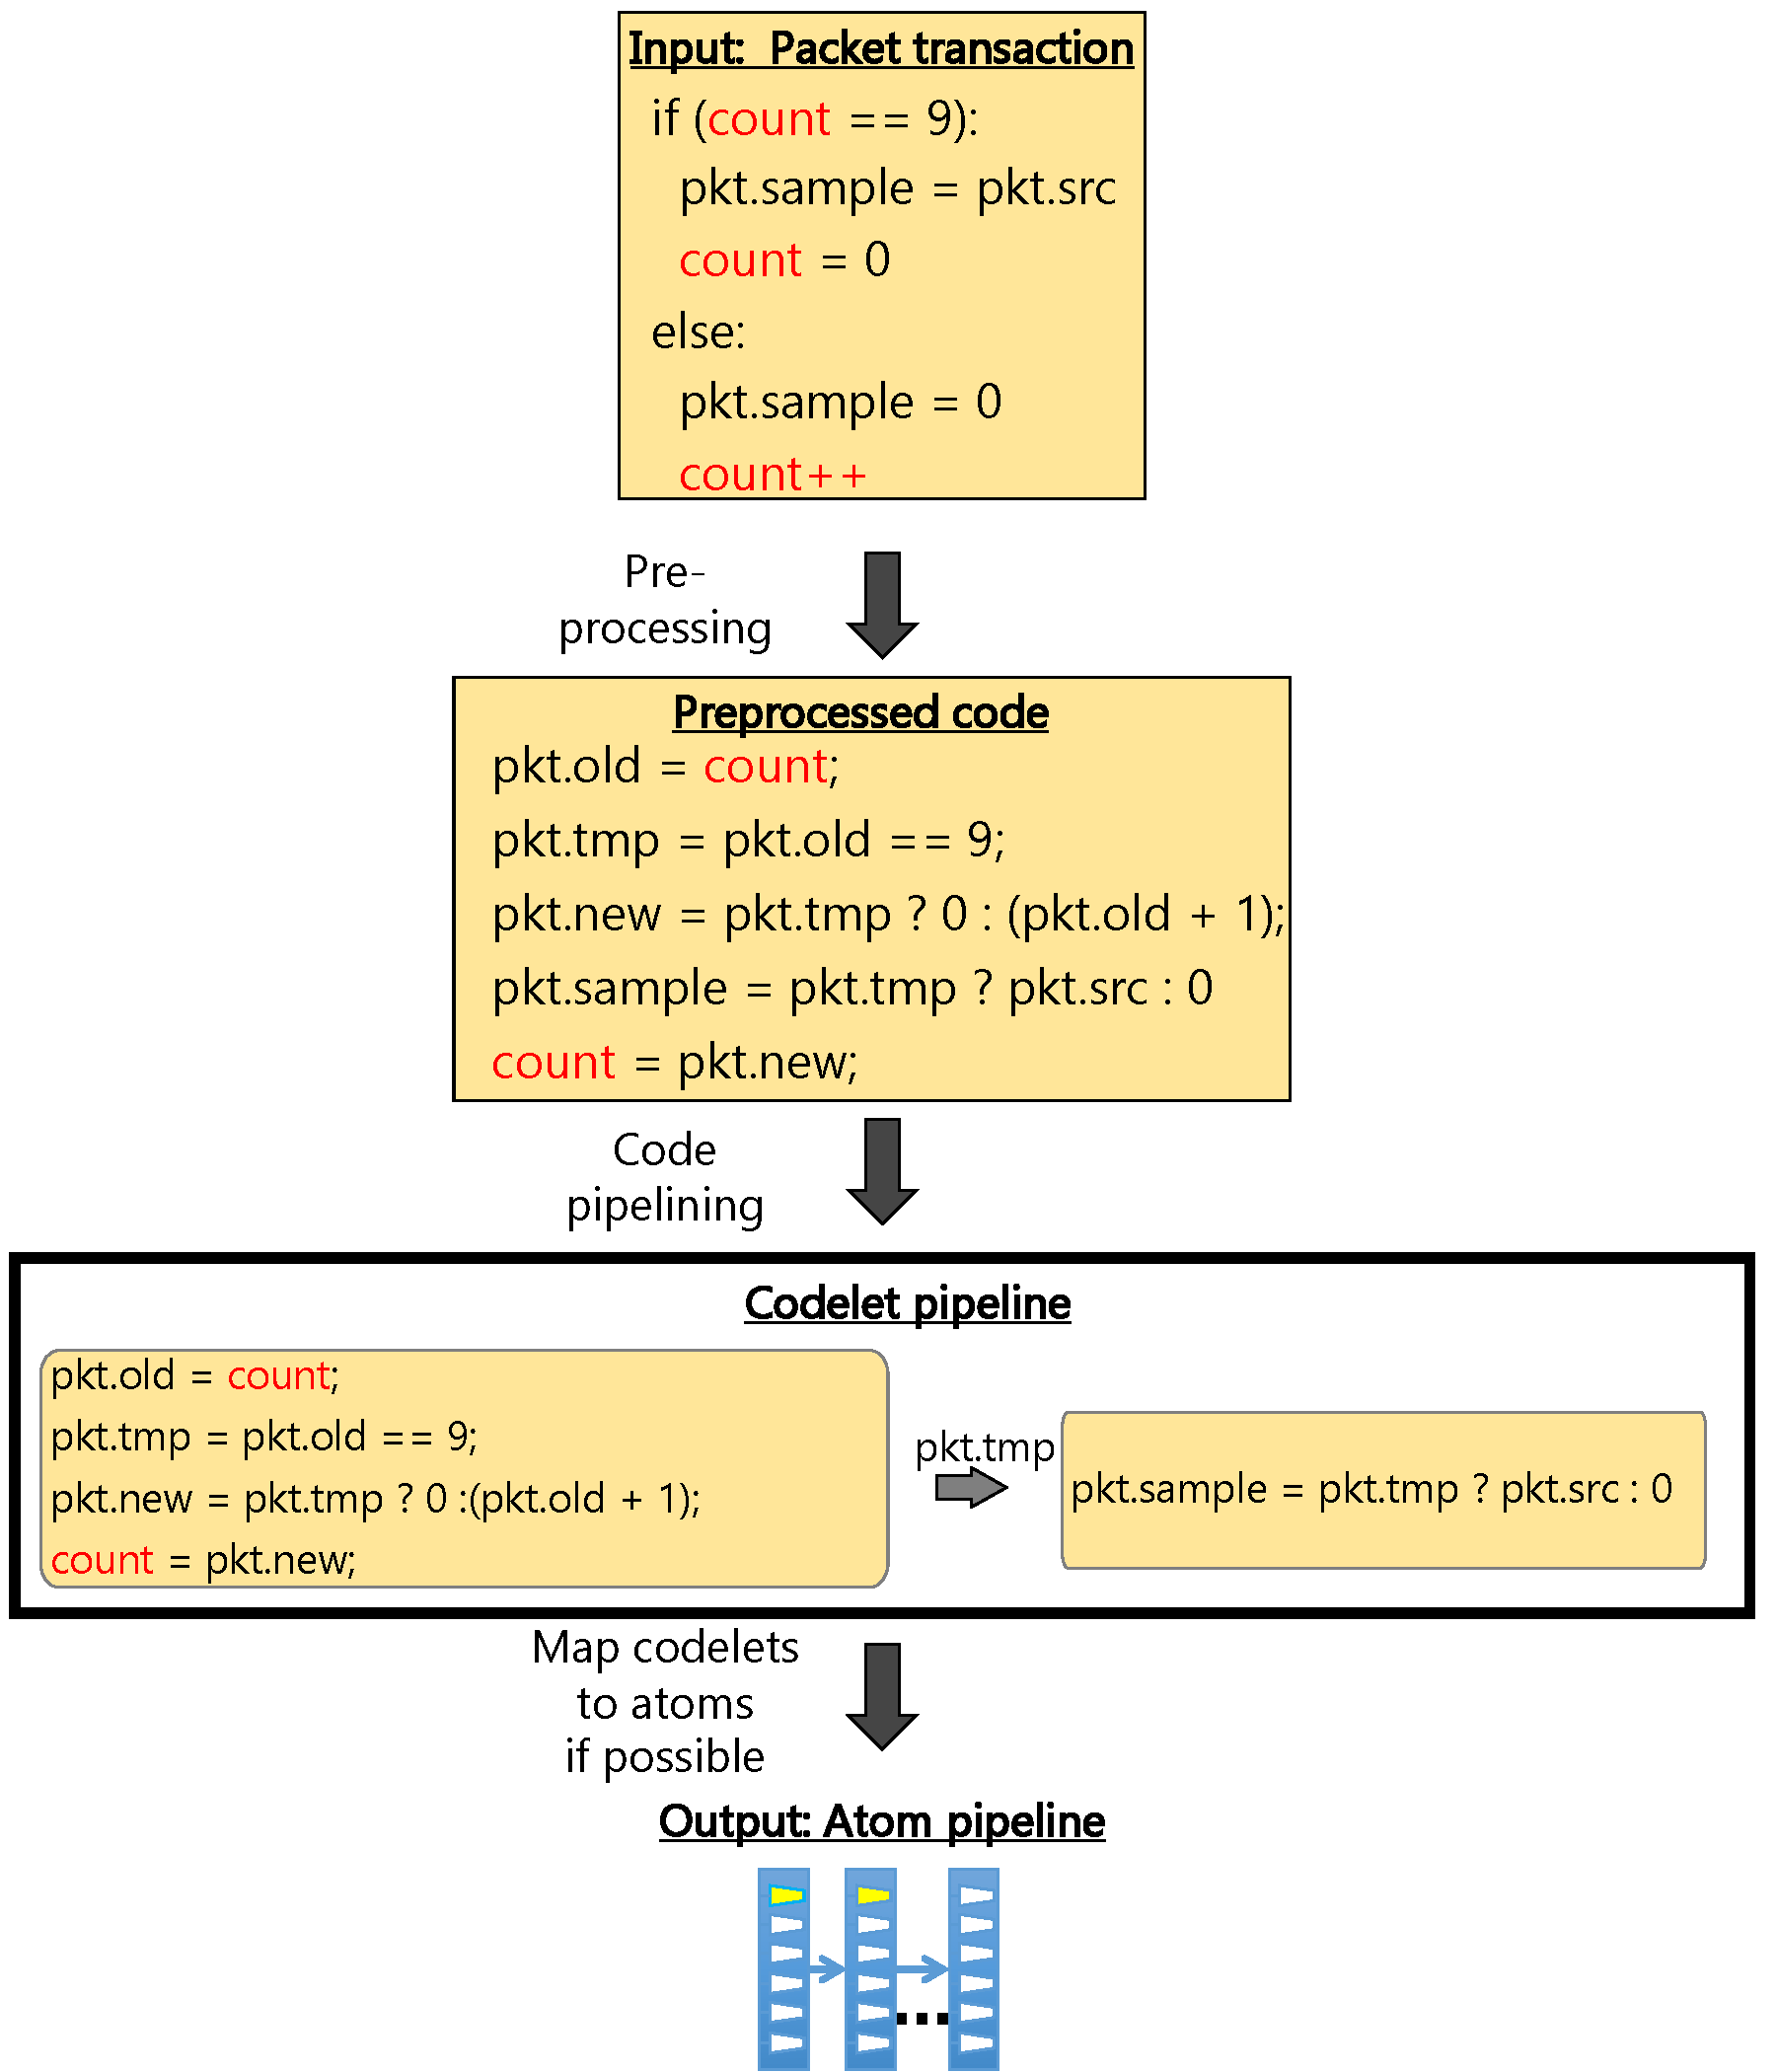
\includegraphics[width=\textwidth]{compiler_passes_example.pdf}
\caption{The three passes of Domino's compiler shown on the packet transaction from Figure~\ref{fig:simple_transaction}.}
\label{fig:compiler_passes_example}
\end{figure}

\begin{figure}
\centering
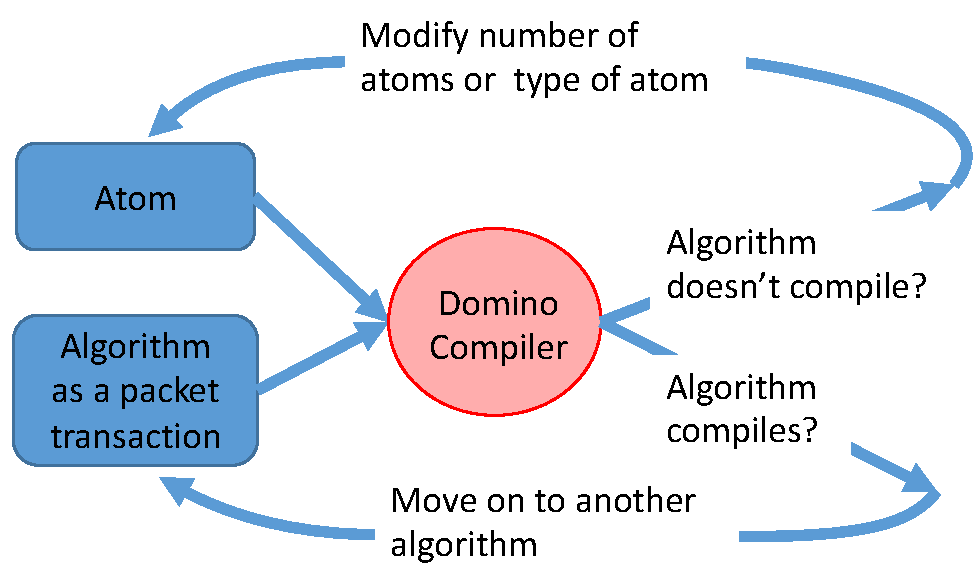
\includegraphics[width=0.4\columnwidth]{iterative_design_process.pdf}
\caption{Iterative atom design process}
\label{fig:iterative_design}
\end{figure}

To develop atoms, we use the Domino compiler to experiment with different atoms
and iteratively modify the atoms until they support enough algorithms
(Figure~\ref{fig:iterative_design}).  Using this process, we developed seven
atoms of increasing complexity (Table~\ref{tab:templates}) that allow us to
progressively program more and more algorithms from
Figure~\ref{fig:router_algos}. For instance, measurement using Bloom filters
only requires simple read and write operations on state. On the other hand,
heavy-hitter detection~\cite{opensketch} uses a counting
sketch~\cite{cormode} that relies on a atomic counter. Finally, algorithms
like flowlet switching~\cite{flowlets} require conditional updates to counters.

In a subsequent project~\cite{perf_query} (Chapter~\ref{chap:perf_query}) that we carried out after
the Domino work, we found that we could reuse the same atoms for other use
cases, providing evidence that these atoms generalize and are useful beyond the
algorithms that influenced their design in the first place.

\subsection{Programmable packet scheduling}
Packet scheduling is an important determinant of network performance. The
choice of scheduling algorithm is tied to a network's overarching goals. For
instance, an algorithm that divides link capacity fairly is ideal in a
multi-tenant setting~\cite{wfq}, while the shortest remaining processing time
algorithm is ideal for a single tenant who desires low flow completion
time~\cite{pFabric}. Today's routers provide a fixed set of scheduling
algorithms. While configuration settings on these scheduling algorithms can be
tweaked, there is no way for an operator to program a new scheduling algorithm
that is tailored to their needs.

Routers lack programmable scheduling because there is no single abstraction to
express many scheduling algorithms~\cite{wfq, srpt, srr, pFabric, lstf}
that appear so different at first brush. This lack of a single unifying
abstraction is not merely an academic concern. It has practical consequences:
in the absence of a single abstraction that can then be hardened in hardware,
we are left with using a general-purpose substrate such as a CPU to program
schedule. As we mentioned earlier, this can seriously hurt performance.

 Push In First Out Queues (PIFOs) (Chapter~\ref{chap:pifo}) provide such an
abstraction.\footnote{PIFOs were first used as a proof construct to establish
the equivalence of combined input-output queued routers and purely output
queued routers~\cite{pifo}. Our contribution is to show that they can gainfully
be used for programmable packet scheduling.} They exploit our observation that
in many practical schedulers, the relative order of packets that are already
buffered does not change in response to new packet arrivals
(\S\ref{s:deconstruct}). Hence, when a packet arrives, it can be pushed into
the right location based on a packet priority (push in), but packets can always
be dequeued from the head (first out). A PIFO is simply a
priority queue of packets with a small program to assign each packet its
priority. Yet, by flexibly programming a packet's priority assignment, a
network operator can use the PIFO abstraction to program a variety of
previously proposed scheduling algorithms. So far, these algorithms could only
be run in simulation or on software routers.

\Para{Programming model for packet scheduling.} Our programming model for
scheduling couples a PIFO with a program to determine a packet's {\em rank} in
the PIFO. This rank can denote the packet's scheduling order (for
work-conserving algorithms such as WFQ) or absolute wall-clock departure time
(for non-work-conserving algorithms such as traffic shaping). This program is
written as a packet transaction, introduced earlier.  Depending on whether the
program determines the scheduling order or time, the program is called either a
scheduling transaction or a shaping transaction.

\begin{figure}
\begin{minipage}[!h]{0.48\textwidth}
\vspace{0.4in}
\begin{lstlisting}[style=customcscriptsize]
f = flow(p) # compute flow from packet p
if f in last_finish:
 p.start = max(virtual_time, last_finish[f])
else: # p is first packet in f
 p.start = virtual_time
last_finish[f] = p.start + p.length/f.weight
p.rank = p.start
\end{lstlisting}
\caption{Scheduling transaction for the Start-Time Fair Queueing implementation~\cite{stfq} of Weighted Fair Queueing.}
\label{fig:wfq_trans}
\hfill
\end{minipage}
\begin{minipage}[!h]{0.48\textwidth}
\begin{lstlisting}[style=customcscriptsize]
tokens = tokens + r * (now - last_time)
if (tokens > B):
  tokens = B
if (p.length <= tokens):
  p.send_time = now
else:
  p.send_time = now + (p.length - tokens) / r
tokens = tokens - p.length
last_time = now
p.rank = p.send_time
\end{lstlisting}
\caption{Shaping transaction for Token Bucket Shaping.}
\label{fig:tbf_trans}
\end{minipage}
\caption{Examples of scheduling and shaping transactions. {\tt p.x} refers to a packet field {\tt x} in packet {\tt p}.  {\tt y} refers to a state variable
that is persisted on the router across packets, \eg {\tt last\_finish}
and {\tt virtual\_time} in this snippet. {\tt p.rank} denotes the
packet's computed rank.}
\end{figure}

A single PIFO coupled with a scheduling or shaping transaction can express many
classical scheduling algorithms, \eg token bucket shaping
(Figure~\ref{fig:tbf_trans}), and weighted fair queueing
(Figure~\ref{fig:wfq_trans}). But, a single PIFO is still restricted to
scheduling algorithms with the property that the relative order of packets that
are already buffered does not change in response to new packet arrivals. A
canonical class of scheduling algorithms that violate this relative order
property is the class of hierarchical scheduling algorithms. A well-known
example of this class is Hierarchical Packet Fair Queueing (HPFQ)~\cite{hpfq},
which first divides up the link's capacity fairly among classes, and then when each
class is scheduled, divides up the class's transmission opportunities fairly
among its constituent flows.

\begin{figure}[!t]
\centering
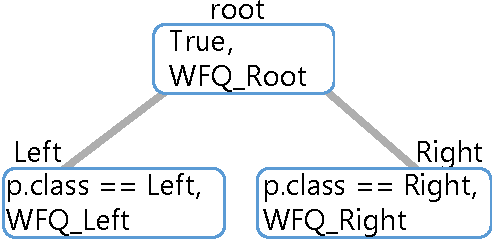
\includegraphics[width=0.5\textwidth]{pifo_hpfq_program.pdf}
\caption{Scheduling tree for HPFQ. The scheduling transactions WFQ\_Root,
WFQ\_Left, and WFQ\_Right are similar to Figure~\ref{fig:wfq_trans} and differ
only in how the flow is computed from the packet. Note that this tree has no
shaping transaction.}
\label{fig:scheduling_tree}
\end{figure}

To support hierarchical scheduling, we extend our programming model from a
single PIFO to a tree of PIFOs, while allowing an entry in a PIFO to be either
a packet or a reference to another PIFO. More formally, a node in a {\em
scheduling tree} (Figure~\ref{fig:scheduling_tree}) has three attributes: (1) a
predicate that determines which packets are handled by that node, (2) a
scheduling transaction that determines a packet's rank in a scheduling PIFO
attached to that node, and (3) an optional shaping transaction that determines
a packet's rank in an optional shaping PIFO.

\begin{figure}[!t]
  \centering
  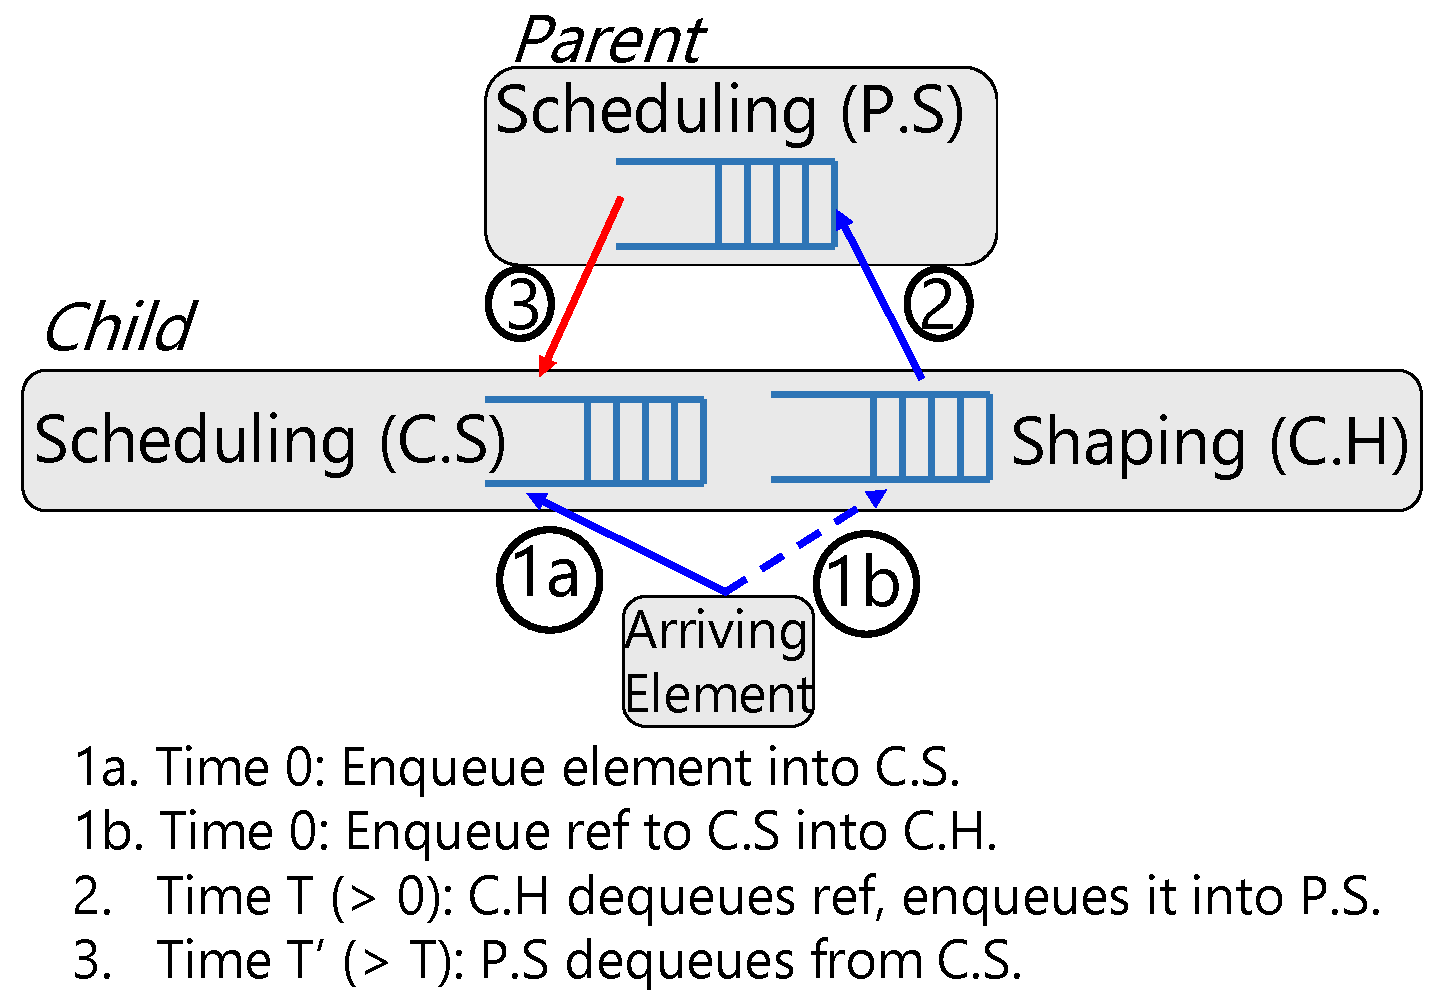
\includegraphics[width=0.6\columnwidth]{pifo_shaping_semantics.pdf}
  \caption{\textit{Child's} shaping transaction (1b) {\em defers} enqueue
  into \textit{Parent's} scheduling PIFO (2) until time T.  Blue arrows
  show enqueue paths. Red arrows show dequeue paths.  }
  \label{fig:shaping_timing}
\end{figure}

We now explain the semantics of a scheduling tree during dequeues and enqueues.
During a dequeue, we walk the scheduling tree starting from the root. We
dequeue the scheduling PIFO at the root, resulting in either a reference to
another scheduling PIFO or a packet. If the result is a packet, we are done,
and we transmit the packet. If not, we continue recursively, dequeueing from
the scheduling PIFO that is pointed to until we find a packet.

When a packet is enqueued, we walk the tree from the leaf whose predicate
captures the packet to the root, executing scheduling and (optionally) shaping
transactions along the way. The scheduling transaction inserts either a packet
or a PIFO reference into the scheduling PIFO. The shaping transaction at a node
inserts a reference to the node's scheduling PIFO in the node's shaping PIFO.
When that reference is dequeued from the shaping PIFO, it is enqueued into the
node's parent's scheduling PIFO. It'll eventually be dequeued from the parent's
scheduling PIFO when it makes its way to the head of the parent's scheduling
PIFO. The shaping PIFO thus provides an optional mechanism to {\em defer}
enqueues into a parent's scheduling PIFO. Figure~\ref{fig:shaping_timing}
illustrates the timing of various operations related to a scheduling and a
shaping PIFO.

The PIFO-based programming model unifies several scheduling algorithms and
allows us to program a wide variety of scheduling algorithms using the single
construct of the push-in first-out queue, \eg Weighted Fair
Queueing~\cite{wfq}, Token Bucket Shaping~\cite{tbf}, Hierarchical Packet
Fair Queueing~\cite{hpfq}, Least-Slack Time-First~\cite{lstf}, the
Rate-Controlled Service Disciplines~\cite{rcsd}, and fine-grained priority
scheduling (\eg Shortest Job First).

\Para{Hardware for PIFOs.} Supporting this programming model is a high-speed
hardware design for PIFOs. When designing hardware for PIFOs, we set out to
meet performance targets that are typical for a single-chip shared-memory
router today. These are routers that are built out of a single
application-specific integrated circuit (ASIC), and whose packet buffer and
scheduling logic is shared across all ports. Sharing the packet buffer and
scheduling logic reduces the memory and digital logic cost associated with
packet scheduling.

For concreteness, we picked a target clock frequency of 1 GHz to reflect a
requirement of performing one enqueue and one dequeue every nanosecond (typical
of high-speed routers today~\cite{rmt}). We targeted a packet buffer of size 12
MByte based on the buffer size of the Broadcom Trident
II~\cite{bcom_buffer}, a recent commercial single-chip shared memory
router. With a cell size of 200 bytes,\footnote{A cell is the minimum unit of
memory allocation in the packet buffer.} a 12 MByte buffer can support up to
60000 packets.

A naive way to implement a 60K-entry PIFO is to use a flat sorted array of 60K
elements and insert an incoming element into this array in a manner reminiscent
of insertion sort. Concretely, an incoming element's rank would be compared in
parallel to the ranks of all 60K elements producing a bitmask denoting which
elements were greater than or lesser than the incoming element. Because the
PIFO is sorted, the bitmask would have a single 0-to-1 transition, the position
of which could be detected using a priority encoder. Finally, the new element
could be inserted into this position. The problem with this approach is that it
is hard to lay out 60K parallel comparators, one for each element in the PIFO.

Instead, we exploit the observation that in most practical scheduling
algorithms, the scheduling is really across flows and not packets, because
packet ranks increase monotonically within a flow to prevent packet reordering
within a flow. Because ranks increase monotonically within a flow, we only need
to look at the first packet of each flow to determine which packet to dequeue
next. This reduces the number of elements that need to be sorted from 60K
packets in the naive implementation to around 1K flows (again, we picked this
number with reference to the Broadcom Trident II that supports \textasciitilde10 queues
on each of its \textasciitilde100 ports).

We find that transistor technology has evolved to the point where it is
relatively cheap to build a sorted array of 1K flows, where a flow can be
enqueued into or dequeued from the array every nanosecond. In a recent
industry-standard 16 nm technology node, a hardware design for a programmable
5-level hierarchical scheduler costs less than 4\% additional chip area
relative to a 200 \si{\milli\meter\squared} baseline router
chip~\cite{glen_parsing}.

\subsection{Scalable network measurement}

Chapter~\ref{chap:perf_query} considers the problem of programmable and
scalable network measurement. Can we have network operators specify the
per-flow statistics they want to measure (\eg a moving average over queueing
latencies or a count of packets or bytes) at the flow granularity they desire
(\eg at the 5-tuple level or at the level of each distinct destination IP
address)? Current router solutions for measurement~\cite{netflow, tetration-telemetry}
fix either the statistics that can be measured or the granularity at which the
statistics can be measured. The challenge here is to provide a set of
measurment primitives that can cover a range of statistics while scaling to a
large number of flows.

\begin{figure}
\begin{minipage}[!h]{\textwidth}
\centering
\begin{lstlisting}
result = filter((*\pktlog,*) qid == Q && tout - tin > 1ms)
// Filter out packets whose queueing delay at queue Q exceeds one ms.
\end{lstlisting}
\end{minipage}

\begin{minipage}[!h]{\textwidth}
\centering
\begin{lstlisting}
result = map((*\pktlog,*) [tin/epoch_size], [epoch])
// Round off packet time stamps to the nearest epoch.
\end{lstlisting}
\end{minipage}

\begin{minipage}[!h]{\textwidth}
\begin{lstlisting}
def count([c], []):
  c = c + 1
result = groupby((*\pktlog{}*), [(*\codeftuple{}*)], count)
// Partition packets by 5-tuple and count the number of packets in each 5-tuple.
\end{lstlisting}
\end{minipage}
\caption{Three example \TheSystem queries. {\ct \pktlog{}} refers to the
original packet performance stream with one tuple for each packet seen in the
network.}
\label{fig:example_queries}
\end{figure}

\Para{Programming model.} To allow network operators to express a wide range of
performance questions, we provide network operators with the abstraction of a
performance packet stream: a stream of tuples, one for each packet, containing
essential information identifying the packet (source and destination address,
source and destination ports) and its performance information (the timestamp at
which the packet was enqueued and dequeued).

Network operators can query this performance packet stream using a functional
query language, \TheSystem, with familiar constructs such as {\ct map}, {\ct
filter}, and {\ct groupby} much like functional APIs in mainstream programming
languages like Python, Java, Scala, and Haskell. Figure~\ref{fig:example_queries}
shows some example queries in \TheSystem. These constructs take as input
a stream of tuples and return an output stream that either transforms each
tuple in the stream ({\ct map}), drops certain tuples based on a predicate
({\ct filter}), or partitions the stream into substreams based on a predicate
and then aggregates the tuples within each substream based on a user-defined
aggregation function ({\ct groupby}).\footnote{Aggregation functions are also
known as fold functions or reduce functions in functional languages.  Our use of user-defined aggregation functions is distinct from the
groupby constructs supported by traditional query languages (\eg SQL). SQL only
supports specific order-independent aggregation functions like counts and
averages, and does not allow general user-defined aggregation functions.}
Because these constructs produce and consume streams, \TheSystem queries can be
easily composed.

\TheSystem allows operators to express both queries that do and do not require
router state to execute. For instance, a stateless {\ct map} query could take
an input packet stream, round off the enqueue timestamp of each packet in the
stream to the nearest millisecond, and return the result as a new stream.  This
query is stateless because it can operate independently on each packet without
maintaining any state on the router that persists between packets. On the other
hand, consider a {\ct groubpy} query that (1) partitions the packet stream into
substreams based on the 5-tuple, and (2) counts the number of packets within
each substream. This query is stateful because it needs to maintain a
dictionary mapping each 5-tuple to its count as persistent router state; this
dictionary is updated by incrementing some 5-tuple's counter on each packet.

\Para{Router hardware for performance queries.}

A naive implementation of the performance query abstraction is to stream out
every packet to a centralized collection server, which executes the performance
query against the incoming packet stream. However, this would require a large
amount of computational resources on the server and almost a dedicated
measurement network to stream every packet to the server. Instead, we use
programmable routers as first-class citizens to perform early filtering,
aggregation, and packet transformations to reduce the amount of data collected
on the collection server.

Supporting stateless queries ({\ct map} and {\ct filter}) is relatively
straightforward. Emerging programmable router chips~\cite{rmt, xpliant,
flexpipe, tofino} already provide an instruction set that performs stateless
manipulations on packet headers. We leverage this instruction set as is to
execute stateless queries.

To support \TheSystem's stateful construct, the {\ct groupby}, we design a
programmable key-value store in hardware. The keys represent the flows and the
values represent the state being aggregated as packets are processed. For
instance, the key could be a 5-tuple and the value could be a count of
bytes/packets belonging to that 5-tuple.

This key-value store has two requirements that are at odds with each other: it
needs to be fast to process packets at the router's line rate (a packet every
nanosecond), and it needs to be large to store a large number of flows. Static
random-access memory (SRAM) can be accessed once every nanosecond, but has low
memory density. On the other hand, dynamic random-access memory (DRAM) has much
better density, but can be accessed once every tens of nanoseconds.

We use caching to support both requirements: a fast SRAM cache stores the
currently active flows, while a backing store in DRAM handles evictions from
the cache. However, cache misses in traditional processor designs lead to
unpredictable memory access latencies while the data is being fetched from the
backing store. A processor handles this by occasionally stalling its pipeline
to handle a cache miss. But stalling a router pipeline prevents us from
providing the deterministic latency guarantees that routers are known for.

\begin{figure}
\centering
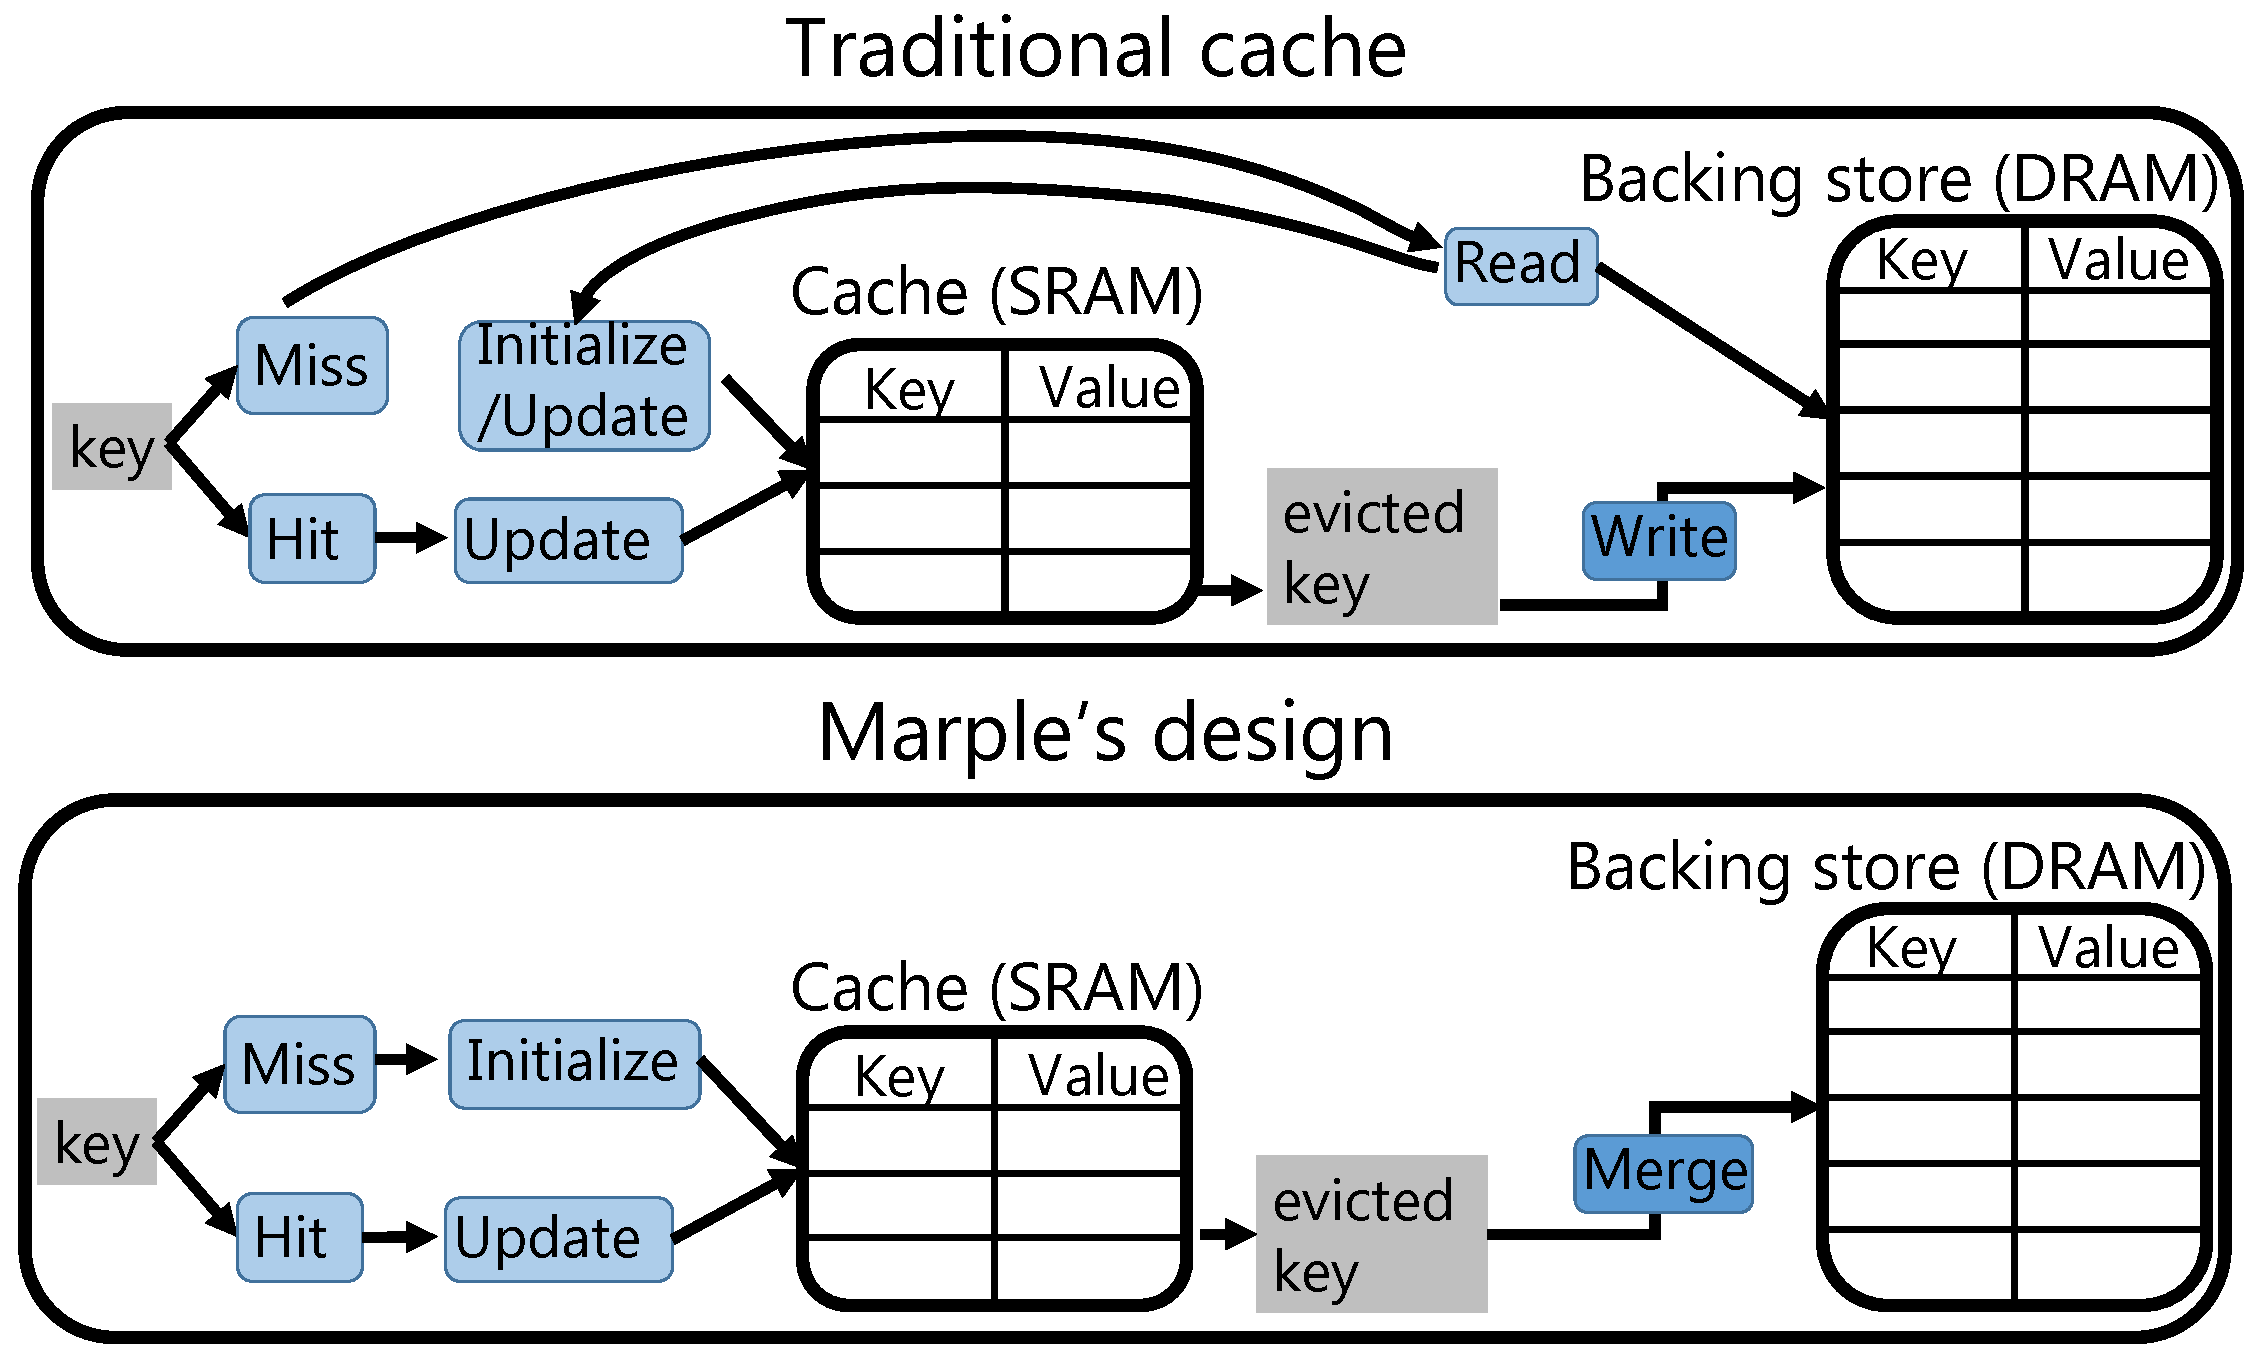
\includegraphics[width=0.6\columnwidth]{pq_kv_store.pdf}
\caption{\TheSystem's key-value store vs. a traditional cache}
\label{fig:hw_diff}
\end{figure}

Instead, as Figure~\ref{fig:hw_diff} shows, we treat a cache miss as the
arrival of a packet from a new flow and initialize the cache entry the way we
would if we had seen a new flow. When this cache entry is eventually evicted,
we merge it against the old value for that entry in the backing store. It is
easy to see that this would work when the value in the key-value store was a
counter; the merge operation would simply add up the old and new counts. But is
merging possible in general?

We formalize characterize a class of aggregation functions for which such
merging is possible without losing accuracy (\ie the value is equivalent to the
value that would be obtained in an ideal system with an infinitely large
cache). We call this class the class the {\em linear-in-state} class because
aggregation functions in this class take on the form:
\begin{equation}
S = A(p) * S + B(p)
\end{equation}
Here $S$ is the state/value that is being updated by the aggregation function,
while $A$ and $B$ are functions of a a bounded number of packets into the past
including the current one. The linear-in-state class captures a variety of
aggregation functions including counters, predicated counters, moving average
filters, and arbitrary functions on sliding windows.

\Para{Evaluation.} We evaluate \TheSystem by expressing several performance
queries: tracking the loss rate on a per-flow basis, measuring the extent of
reordering in a TCP flow, measuring a moving average of queueing latencies on a
per-flow basis, and detecting the presence of TCP incast. Our \TheSystem
compiler compiles these queries to two different targets: an atom pipeline to
determine the hardware feasibility of \TheSystem queries and a P4-based
software switch~\cite{p4-bmv2} for end-to-end case studies of \TheSystem
in Mininet~\cite{mininet}. We find that \TheSystem queries occupy a small
fraction of the router's hardware resources, both computationally in terms of
the number of atoms they need, and memory-wise in terms of the size of the SRAM
cache for our programmable key-value store. We find that the eviction rate from
the SRAM cache is modest: a single 8-core server running REDIS~\cite{redis} can
support the typical eviction rate from a 64-port switch with 10 Gbit/s links.
Our Mininet experiments show that \TheSystem can be used to iteratively
troubleshoot problems such as occasional latency spikes happening as a result
of bursty background traffic.

\section{Lessons learned} We conclude this chapter by distilling some general
lessons for programmable router design that go beyond the specific
contributions of each of the three systems.

\Para{The power of specialization.} The most important lesson here  is the
power of specialization: the idea of targeting hardware and software to
specific classes of router functionality.  The three systems in the
dissertation demonstrate how narrowing our focus to specific router
functionality allows us to resolve the performance-programmability tradeoff
that has plagued routers so far.

In the language of computability, none of our systems is Turing-complete: they
cannot simulate a Turing machine, an idealization of the general-purpose CPU.
We refer the reader to \S\ref{domino_ss:limitations} and
Table~\ref{tab:restrict}, \S\ref{pifo_ss:limitations}, and
\S\ref{sec:compiler} for specific examples of what each of the three
systems cannot express.
%TODO: Change reference to Marple limitations once we put in the new text from
%the SIGCOMM camera ready.

Yet, each covers a large number of example use cases within specific
functionality classes (stateful data-plane algorithms, scheduling, and
measurement queries) without giving up performance relative to a fixed-function
router. Viewed differently, by specializing, each system provides an order of
magnitude improvement in performance relative to a general-purpose software
router. Intellectually, these results suggest that there is a rich space of
system designs that is as yet unexplored---if we choose to look beyond
Turing-complete systems. 

\Para{Jointly designing hardware and software.} We are entering an era where
Moore's law has slowed down or effectively stopped~\cite{dark_silicon,
four_horsemen}.  In this new era, transistors are no longer guaranteed to get
smaller or faster every year. In the heyday of Moore's law, processor hardware
automatically got faster year on year, and software automatically enjoyed the
free lunch of improved performance because of the underlying improvements in
hardware. With the end of Moore's law, it is no longer apparent how these
performance improvements will be sustained.

Jointly designing hardware and software in service of a higher-level
application-level goal suggest a way to continue improving performance. Year on
year, the greatest performance improvements will come from human creativity in
specializing hardware to specific application needs and then appropriately
exposing this specialized hardware to software. This is already visible in
domains such as machine learning. For instance, the tensor processing
unit~\cite{tpu} is an ASIC tailored to deep learning, and
TensorFlow~\cite{tensorflow} is its corresponding programming model.

The systems presented in this dissertation are also examples of joint hardware
and software design in the context of networking, where we develop both the
underlying hardware (atoms, PIFOs, and hardware key-value stores) and the
corresponding software (packet transactions, scheduling trees, and performance
queries) for specific application classes (stateful data-plane algorithms,
scheduling, and statistics measurement).

\Para{Vertically integrated thinking.} Philosophically, the results in the
dissertation advocate for vertically integrated thinking, where a single system
design incorporates the entire computing stack starting with programmable
hardware, up through the compiler for this hardware, and finishing off with the
language to program this hardware. For decades now, systems programmers have
treated the hardware as programmable, but unmodifiable. There are undeniable
benefits to writing software for off-the-shelf commodity hardware because it is
immediately deployable---in contrast to vertically integrated systems that need
to be first designed in hardware and then programmed in software. At the same
time, the results here suggest that there are substantial performance benefits
from redesigning the entire stack from the ground up.
